%!TEX root = ../main.tex

\section{Implementation} % (fold)
\label{sec:implementation}


\subsection{Visual Implementation} % (fold)
\label{sub:visual_implementation}

% subsection visual_implementation (end)


\subsection{Sound Implementation} % (fold)
\label{sub:sound_implementation}

\begin{enumerate}
    \item Input Sound
    \item Array / Sample
    \item Determine Sample Speed
    \item Phasor
    \item Merge Array and Sample Speed
    \item Fliter
    \item Output Sound
    \item Tracker
\end{enumerate}

Here is a overview of one of the pure data systems that has been made:

\begin{figure}[!htbp]
    \centering
    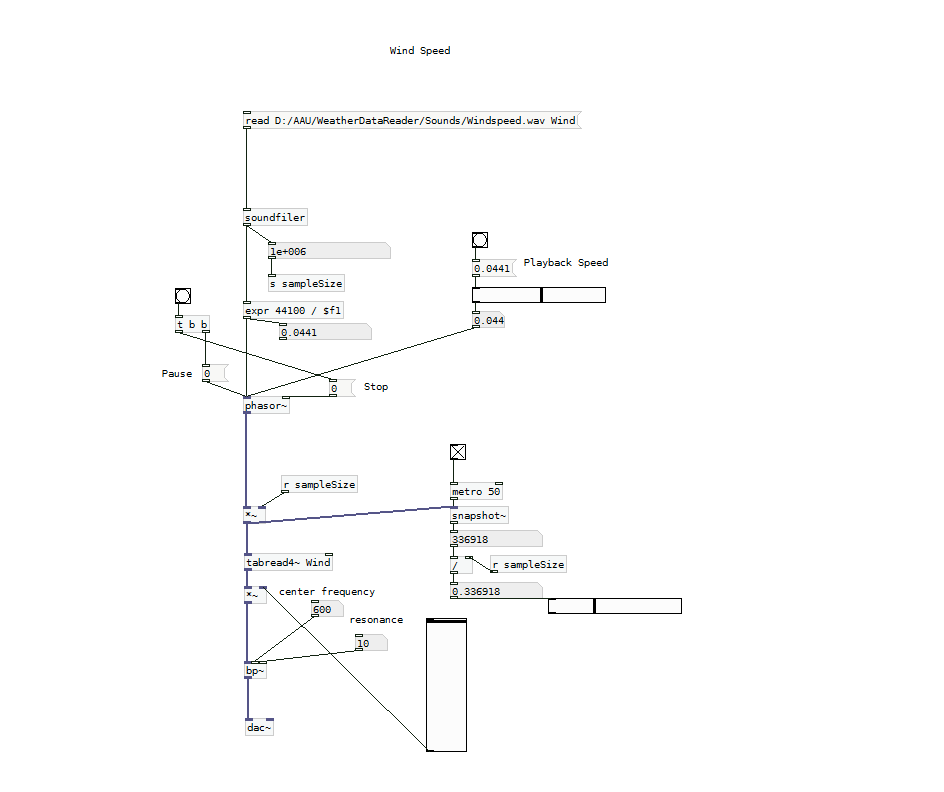
\includegraphics[width=1\textwidth]{images/Implementation1.png}
    \caption{Sample Pure Data implementation}
    \label{fig:implementation1}
\end{figure}


\subsubsection*{Step 1} % (fold)
\label{ssub:step_1}

Here the program reads where the sound is placed on the computer and imports it into an array. 
As seen on the figure~\ref*{fig:implementation2} the path have been written down and in this case the array is called Wind.

\begin{figure}[!htbp]
    \centering
    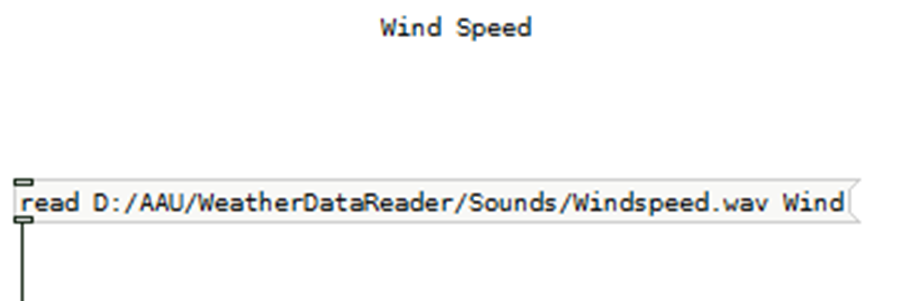
\includegraphics[width=.7\textwidth]{images/Implementation2.png}
    \caption{Sample audio import}
    \label{fig:implementation2}
\end{figure}

This is the array itself (Figure~\ref{fig:implementation3}). 
Here you can see what the different sound waves are going to look like. 
It might seem when you look at the arrays that there is a lot of wasted space in the array. 
This is simply because some of the sound don’t last that long and the empty space you see in the array is lesser than a second when played.

\begin{figure}[!htbp]
    \centering
    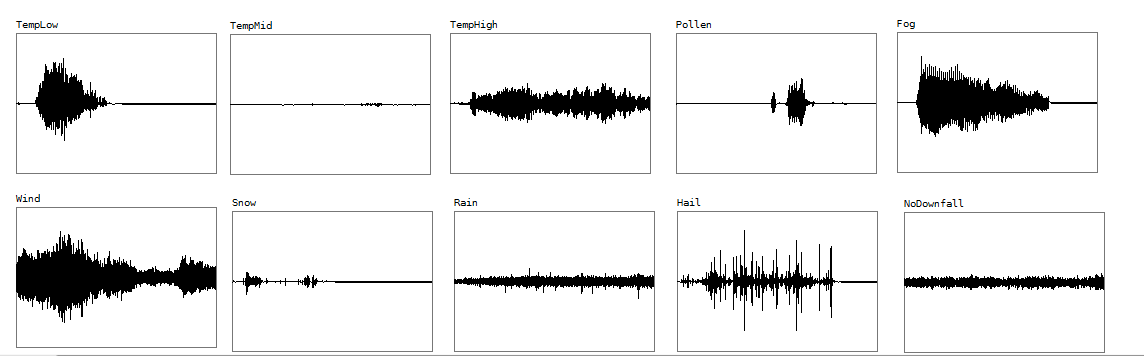
\includegraphics[width=.5\textwidth]{images/Implementation3.png}
    \caption{Sound sample array}
    \label{fig:implementation3}
\end{figure}

% subsubsection step_1 (end)


\subsubsection*{Step 2} % (fold)
\label{ssub:step_2}

Here the soundfiler collects the amount of samples and the speed. 
As seen on the picture (Figure~\ref{fig:implementation4}) the sample amount is been read and stored in sampleSize that will be used later in the program. 
The data follows the path down to the phasor.

\begin{figure}[!htbp]
    \centering
    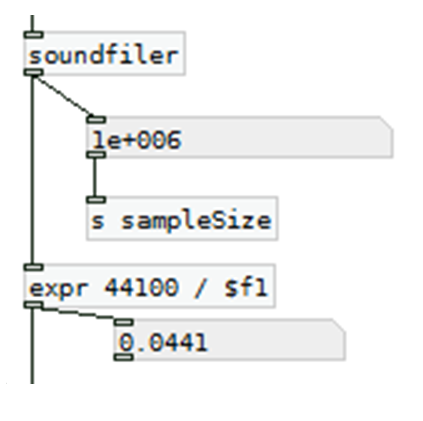
\includegraphics[width=.3\textwidth]{images/Implementation4.png}
    \caption{Soundfiler implementation}
    \label{fig:implementation4}
\end{figure}

% subsubsection step_2 (end)


\subsubsection*{Step 3} % (fold)
\label{ssub:step_3}

We made a system that can control the speed of the samples. 
Here we can replace the original speed with our own to change the speed of the sound. 
This is done in the box you see right besides the text Playback Speed on the picture (Figure~\ref{fig:implementation5}).

\begin{figure}[!htbp]
    \centering
    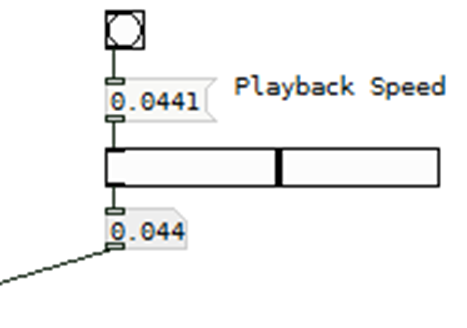
\includegraphics[width=0.3\textwidth]{images/Implementation5.png}
    \caption{Playback speep sample}
    \label{fig:implementation5}
\end{figure}

% subsubsection step_3 (end)


\subsubsection*{Step 4} % (fold)
\label{ssub:step_4}

Here is all the information sent to the phasor that carries the new information over to the next step that is merging with the array.

\begin{figure}[!htbp]
    \centering
    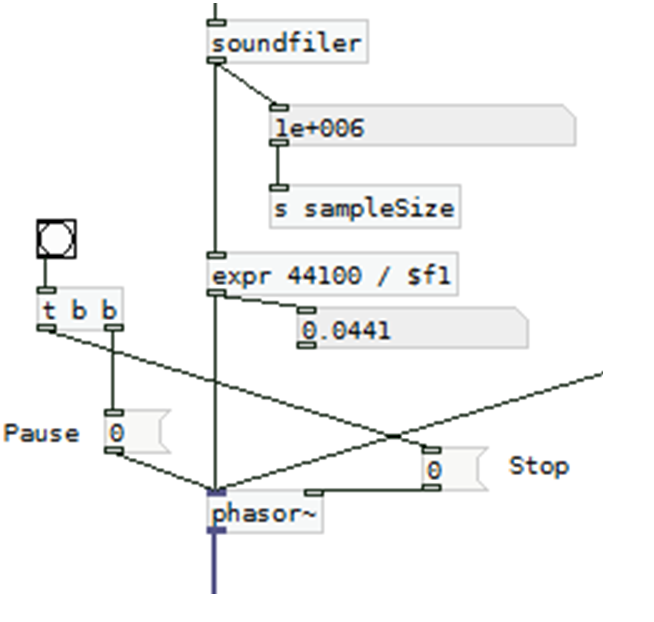
\includegraphics[width=0.3\textwidth]{images/Implementation6.png}
    \caption{Phasor}
    \label{fig:implementation6}
\end{figure}

% subsubsection step_4 (end)


\subsubsection*{Step 5} % (fold)
\label{ssub:step_5}

Here (Figure~\ref{fig:implementation7}) it loads the old array with the new changes to the sound. 
At this point the play speed has been changed and changes to the sound has been made.

\begin{figure}[!htbp]
    \centering
    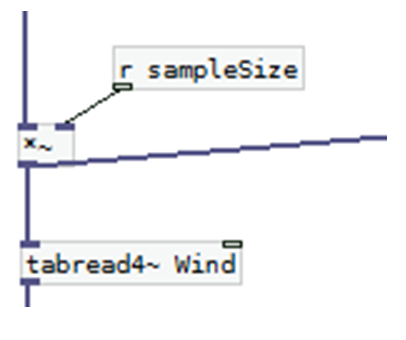
\includegraphics[width=0.3\textwidth]{images/Implementation7.png}
    \caption{Load old array}
    \label{fig:implementation7}
\end{figure}

% subsubsection step_5 (end)


\subsubsection*{Step 6} % (fold)
\label{ssub:step_6}

Here is our bp\~ filter as seen the two boxes linked to the filter are the center frequency and the resonance. 
In this case the center frequency is 600 and the resonance is 10.

\begin{figure}[!htbp]
    \centering
    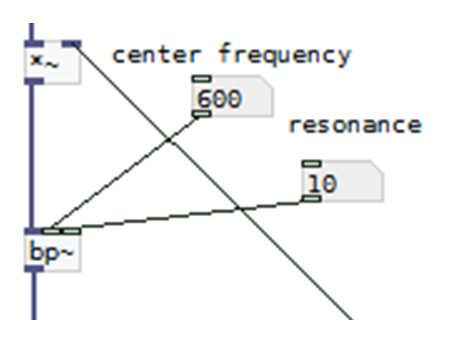
\includegraphics[width=0.3\textwidth]{images/Implementation8.png}
    \caption{bp Fliter}
    \label{fig:implementation8}
\end{figure}

% subsubsection step_6 (end)


\subsubsection*{Step 7} % (fold)
\label{ssub:step_7}

After the filter all the information is sent to dac\~ which is the audio output.

\begin{figure}[!htbp]
    \centering
    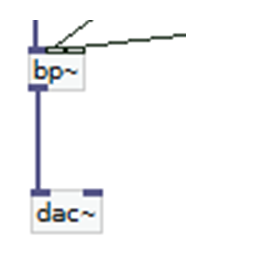
\includegraphics[width=0.3\textwidth]{images/Implementation9.png}
    \caption{dac output}
    \label{fig:implementation9}
\end{figure}

% subsubsection step_7 (end)


\subsubsection*{Step 8} % (fold)
\label{ssub:step_8}

Additional feature:

There was also implemented a length tracker in order to know when the sound clip was done playing. 
This didn’t change the sound at all but it can be nice for us during testing.

\begin{figure}[!htbp]
    \centering
    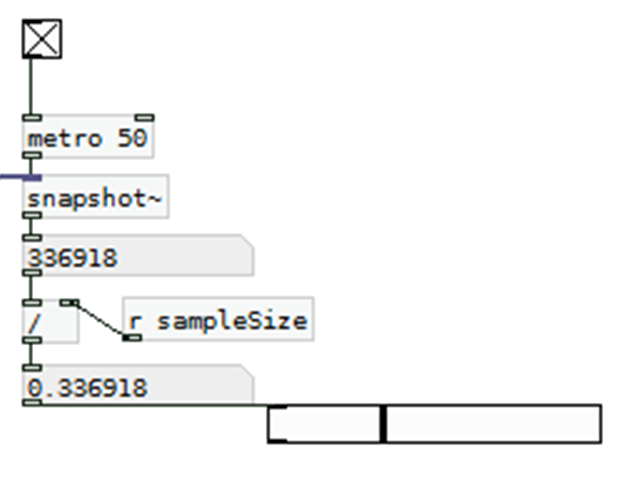
\includegraphics[width=0.3\textwidth]{images/Implementation10.png}
    \caption{Length Tracker}
    \label{fig:implementation10}
\end{figure}

% subsubsection step_8 (end)

% subsection sound_implementation (end)

% section implementation (end)